\chapter{Convex Conjugates}
\label{chap:convex_conjugates}

\section{Definition and properties}

This chapter introduces a concept that is deeply connected to subgradients and
proximal mappings (as covered in the last two chapters), and to duality theory
(as will be covered next). In fact, just as with subgradients, proximal
mappings, and duality, the topic of the current chapter is both simple and
elementary and at the same time highly significant and powerful.    

Given a function $f$ on $\R^d$, its \emph{convex conjugate} $f^*$ (also simply
called its conjugate) is another function on $\R^d$ defined as    
\index{convex conjugate}
\index{Legendre-Fenchel transform}
\begin{equation}
\label{eq:convex_conjugate}
f^*(u) = \sup_x \, \Big\{ u^\T x - f(x) \Big\}.
\end{equation}
The mapping from $f \mapsto f^*$ is also called the \emph{Legendre-Fenchel
  transform}. At the outset, we remark that $f^*$ is always convex, by the
partial supremum rule in Property \parref{par:function_supremum} (the map
$u \mapsto u^\T x - f(x)$ is convex---indeed, it is affine---for each $x$). To
be clear, this is true regardless of the convexity of $f$, which is why $f^*$ is 
called its convex conjugate.  

An interpretation of the convex conjugate $f^*$ is as follow: at each point $u$,
the value $f^*(u)$ is the maximum gap between a linear function with ``slope''
$u$ and $f$. Figure \ref{fig:convex_conjugate} gives an illustration.    

\begin{figure}[tb]
\centering
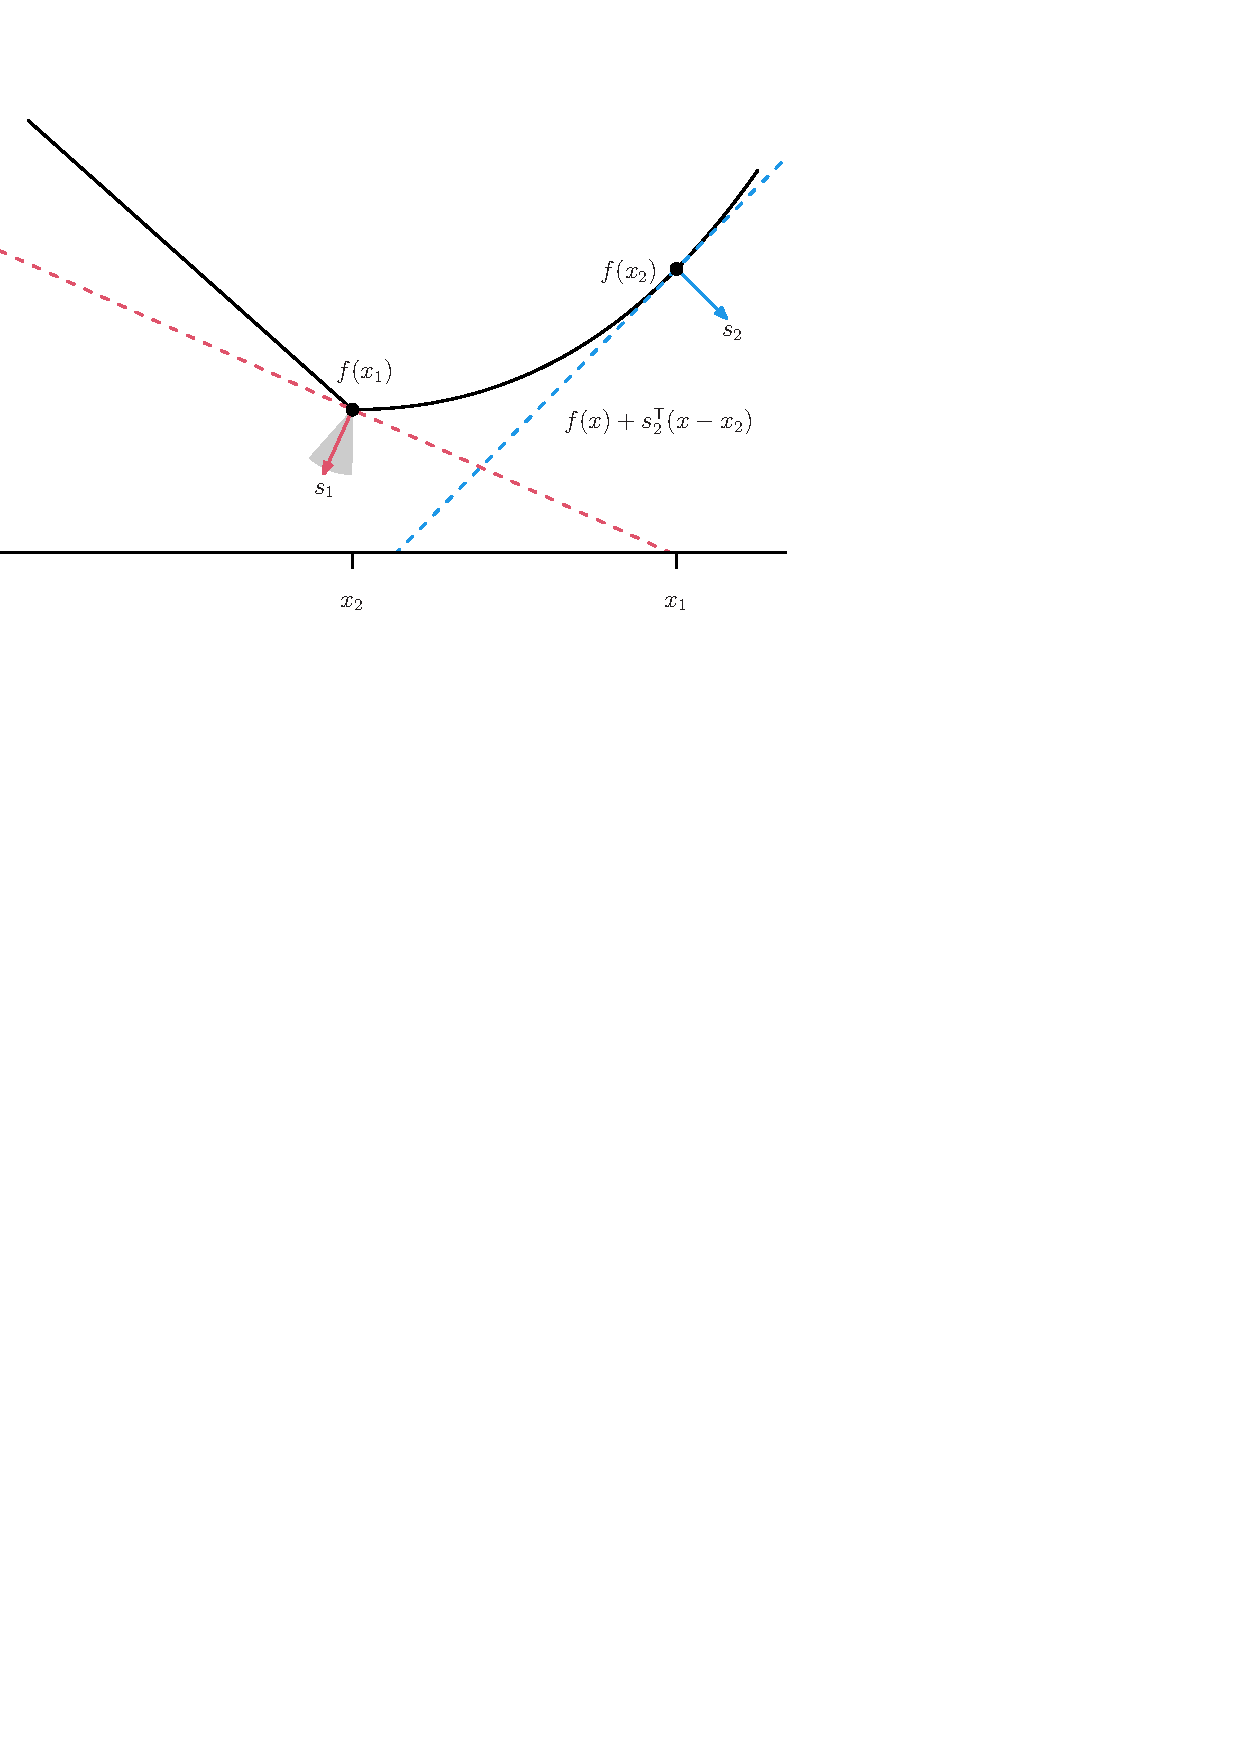
\includegraphics[width=0.7\textwidth]{fig/subgradient.pdf}
\caption{Two example subgradients $s_1$ and $s_2$ of a function $f$ at two
  points $x_1$ and $x_2$, respectively. Each $s_i$ defines a linear map 
  that passes through $x_i$ and lies below $f$ everywhere (that is, it defines a
  supporting hyperplane to $\epi(f)$ at $x_i$, whose normal is $(s_i,-1)$). At
  $x_2$, $f$ is differentiable, and $s_2 = \nabla f(x_2)$ is the only
  subgradient; at $x_1$ there are many possible subgradients (as illustrated
  by the gray wedge).}
\label{fig:convex_conjugate}
\end{figure}

Now we describe several important properties of convex conjugates. 

\paragraph{Fenchel's inequality.}

\paragraph{Double conjugation.}

conjugates and subgradients---where does this go?

what else?

examples

\section{Conjugate calculus}

should check rockafellar and bertsekas

\section{Conjugates and smoothness*}
\label{sec:conjugates_smoothness}

discuss relationships between smoothness of f, f* 

define Legendre function (essential smoothness, essential strict convexity).
gradient map is a homeomorphism (with inverse being graident of conjugate) 

\section{Proximal connections*}

\subsection{Moreau decomposition}
\label{sec:moreau_decomposition}

\subsection{Moreau envelope, revisited}

The connection between the moreau envelope and regularization is due to Hedy
Attouch in 1977  

infimal convolution and conjugates and addition

relationship between conjugates and moreau envelopes, which shows it as a form
of smoothing 

\begin{xcb}{Exercises}
\begin{enumerate}[label=\thechapter.\arabic*]
\settowidth{\leftmargini}{0.00.\hskip\labelsep}
\item \label{ex:conjugates_smoothness}

\item linf proximal mapping from Moreau decomposition

\item Operator norm proximal map from linf and Exercise
  \ref{ex:matrix_norm_proximal_mapping2}   

\end{enumerate}
\end{xcb}
